% nastavenia prostredia
\documentclass[12pt,a4paper,titlepage,final]{report}
\usepackage[utf8]{inputenc}
\usepackage[T1, IL2]{fontenc}
\usepackage{graphicx}
\usepackage{epstopdf}
\usepackage[margin=2cm]{caption}
\usepackage[top=3cm, left=2cm, right=2cm, text={17cm, 24cm}, ignorefoot]{geometry}
\usepackage{color}
\usepackage{url}
\usepackage[bookmarksopen,colorlinks,plainpages=false,urlcolor=blue,unicode]{hyperref}
\usepackage{setspace}
\usepackage[czech]{babel}
\singlespacing

\begin{document}
	% define
	\def\authora{Jan Bureš}
	\def\authorb{Pavel Macenauer}
	\def\emaila{xbures19@stud.fit.vutbr.cz}
	\def\emailb{xmacen02@stud.fit.vutbr.cz}
	\def\docname{Počítačová grafika}
	\def\projname{Raytracing na CUDA}
	% titulna strana
	\begin{titlepage}

\vspace*{1cm}

\begin{figure}
  \centering
  
\includegraphics[height=6cm]{images/fit.pdf}
\end{figure}

\vspace*{5mm}

\begin{center}
\begin{Large}
Projekt do předmětu PGR -- Počítačová grafika
\end{Large}
\end{center}

\vspace*{5mm}

\begin{center}
\begin{Huge}
CUDA Raytracer \\
\end{Huge}
\end{center}

\vspace*{1cm}

\begin{center}
\begin{Large}
\today
\end{Large}
\end{center}

\vfill

\begin{flushleft}
\begin{large}
\begin{tabular}{ll}

\bf Řešitelé:\hspace{3mm}
& Jan Bureš (\verb_xlogin00@stud.fit.vutbr.cz_) \\
& Pavel Macenauer (\verb_xmacen02@stud.fit.vutbr.cz_) \\
& Fakulta Informačních Technologií \\
& Vysoké Učení Technické v~Brně

\end{tabular}
\end{large}
\end{flushleft}

\end{titlepage}

% vim:set ft=tex expandtab enc=utf8:

	% kapitoly
	\newpage
	\pagestyle{plain}
	\pagenumbering{arabic}
	\setcounter{page}{1}
	\setcounter{secnumdepth}{-1}
	\setlength{\parindent}{1cm}	

%---------------------------------------------------------------------------
\section{Zadání}

\begin{itemize}
	\item Implementace Raytraceru pomocí technologie CUDA v následujícím rozsahu:
	\begin{itemize}
		\item Geometrická primitiva: roviny, koule
		\item Phongův osvětlovací model
		\item Bodové zdroje světla a stíny
		\item Odlesky
	\end{itemize}
	\item Akcelerace výpočtu scény
	\begin{itemize}
		\item průzkum akcelerace raytracingu na GPU
		\item subsampling
		\item využití akcelerační struktury pro výpočet (BVH, KD-tree, octree, ...)
	\end{itemize}
	\item Vygenerování demonstrační scény a její vykreslení
\end{itemize}

%---------------------------------------------------------------------------
\section{Použité technologie}

\subsection{Technologie potřebné pro spuštění programu:}
\begin{itemize}
	\item CUDA 3.0
	\item OpenGL 4
	\item GLM
	\item Glut
	\item Glew
\end{itemize}
\subsection{Při tvorbě jsme použili tyto programy:}
\begin{itemize}
	\item Visual Studio 2012 + NSight
	\item GitHub
\end{itemize}
%---------------------------------------------------------------------------
\section{Použité zdroje}

\subsection{Studijní zdroje:}
\begin{itemize}
	\item Přednáška PGR (Realistické zobrazování I - Ray Tracing)
	\item \href{https://www.fit.vutbr.cz/study/courses/PGR/private/Aurelius.zip}{Ray-tracer Aurelius}
	\item Přednáška PGP (Fotorealistcké zobrazování, optimalizace sledování paprsku)
	\item \href{http://docs.nvidia.com/cuda}{CUDA Toolkit Documentation}
\end{itemize}

\subsection{Doplňujicí zdroje:}
\begin{itemize}
	\item \href{http://cs.wikipedia.org/wiki/Phong%C5%AFv_osv%C4%9Btlovac%C3%AD_model}{Phongův osvětlovací model}
	\item \href{http://stackoverflow.com/questions/19013156/how-does-cuda-4-0-support-recursion}{Rady ohledně rekurze v CUDA}
	\item \href{http://www.3dmuve.com/3dmblog/?p=182}{Bounding Volume Hierarchies (BVH) – A brief tutorial on what they are and how to implement them}
	\item \href{http://cuda-programming.blogspot.cz/2013/01/what-is-constant-memory-in-cuda.html}{What is constant memory in CUDA?}
	\item \href{http://cg.alexandra.dk/2009/08/10/triers-cuda-ray-tracing-tutorial/}{Triers CUDA ray tracing tutorial}
\end{itemize}
%---------------------------------------------------------------------------
\section{Nejdůležitější dosažené výsledky}

\subsection{Scéna}
\begin{itemize}
	\item 50 koulí
	\item 4 roviny
	\item 1 lesklý materiál
	\item 1 bodové světlo
\end{itemize}

\begin{center}

	\captionsetup{type=figure}
		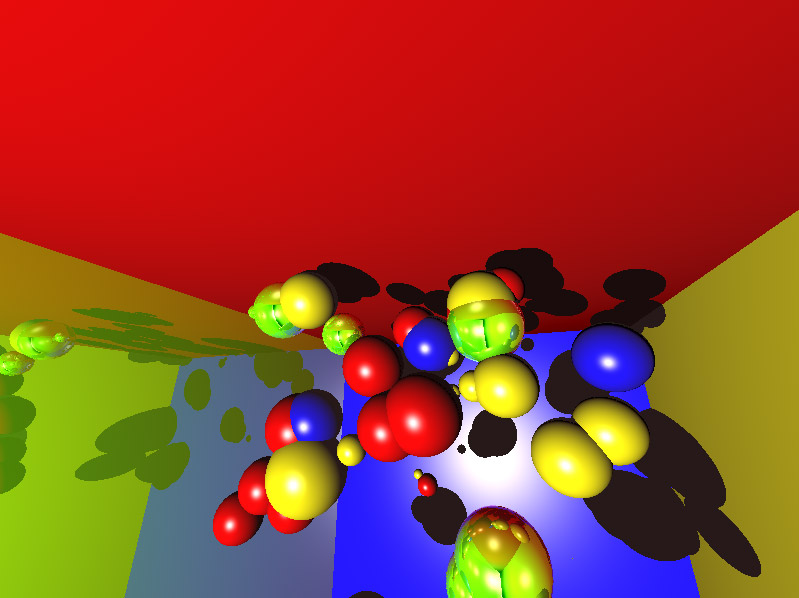
\includegraphics[width=14cm]{images/no-sampling-no-bvh.jpg}
	\captionof{figure}{Vygenerovaná scéna bez využití jakéhokoliv urychlení}
	

	\captionsetup{type=figure}
		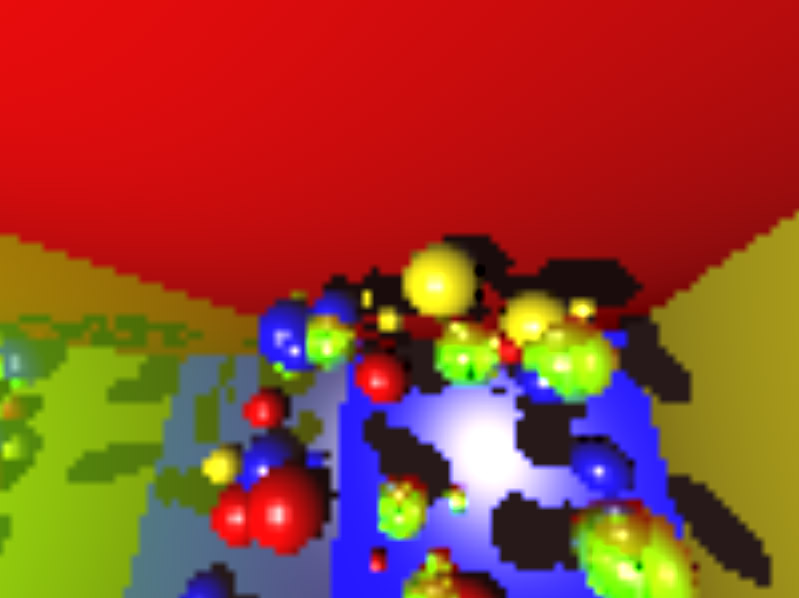
\includegraphics[width=14cm]{images/with-sampling-no-bvh.jpg}
	\captionof{figure}{Vygenerovaná scéna s využitím bilineární interpolace}
\end{center}
	\vspace{5mm}
Jedním z nápadů jak urychlit běh programu výpočtu bylo využít vzorkování/samplingu. Při výpočtu se inicializuje paprsek a následně výpočetní vlákno (thread) pro každý obrazový bod, jejich počet je tak roven ŠÍŘKA OBRAZU * VÝŠKA OBRAZU. 
	
	Při klasickém raytracingu na CPU, lze urychlit běh programu tak, že se nevyšle takto paprsek pro každý bod, ale třeba jen pro každý 8-smý a v případě, že paprsek trefí stále stejné primitivum, tak se barvy mezi těmito body interpolují. V opačném případě se pak vyšlou paprsky pro všechny body neb se jedná o rozhraní mezi 2-mi primitivy.
	
	Na GPU je ten problém, že veškeré výpočty probíhají paralelně a jakékoliv podmínky dramaticky snižují výkonnost. Není tak jednoduše možné říct, kdy vyslat všechny paprsky a kdy jen některé, protože se paprsky posílají po skupinách. Optimalizaci jsme tak provedli pomocí bilineárního interpolování, kdy ve směru jak osy X, tak osy Y vyšleme počet paprsků dělený předem danou konstantou (na Obrázku 2. je hodnota konstanty 8), čímž snížíme počet výpočetních vláken druhou mocninou konstanty.
	
	Vypočtené hodnoty následně uložíme do sdílené paměti v rámci jednoho warpu a pro celý obraz hodnoty dopočteme pouze z těchto vzorků. Výsledný obraz je však výrazně nižší kvality, než-li obraz vygenerovaný bez použití interpolace.


\subsection{Měření na NVidia Quadro K1000M}
\begin{itemize}
	\item CUDA Processing cores: 192
	\item Memory: 2 GB
	\item Memory bandwidth: 29 GBps 
\end{itemize}	
	
\begin{table}[h!]
	\begin{center}
    \begin{tabular}{ | p{3.5cm} | p{3.5cm} | p{3.5cm} | p{3.5cm} |}
    \hline
    Rozlišení & Prům. doba běhu kernelu bez BS [s]& konst=4 [s]& konst=8 [s]
    \\ \hline
    
	1600x800 & 0.1065 & 0.0199 & 0.0068
	\\ \hline
	
	800x600 & 0.0495 & 0.0070 & 0.0030
	\\ \hline
	
    \end{tabular}
	\end{center}	
	\caption{Doba běhu kernelu}  
\end{table}


%---------------------------------------------------------------------------
\section{Ovládání vytvořeného programu}

Program se spustí přes RayTracer.exe s tím, že v konzoli se vypisují hodnoty doby výpočtu kernelu v sekundách.

Při kompilaci lze zapnout/vypnout v souboru \verb|constants.h| parametry se kterými se scéna vypočítává:
\begin{itemize}
	\item \verb|NUM_SPHERES| počet koulí ve scéně pro zvýšení komplexity
	\item \verb|BILINEAR_SAMPLING| využití bilineární interpolace
	\item \verb|SUB_CONST| konstanta, kterou se redukuje počet vláken při bilineárním interpolování
	\item \verb|USE_BVH| využití Bounding Volume Hierarchy
\end{itemize}

%---------------------------------------------------------------------------
\section{Zvláštní použité znalosti}

\subsection{NVidia CUDA}
Hlavní co jsme museli nastudovat jsou vědomosti ohledně technologie CUDA tedy struktura pamětí, jak je používat pomocí jejího C++ API a v kombinaci s programováním na CPU.

K debugování a programování jsme následně využívali vývojové prostředí Microsoft Visual Studio 2012 s NVidia NSight.

Museli jsme nastudovat i témata neprobíraná, resp. jen z lehka naťuklá na přenáškách. Jedním z nich je akcelerační struktura zvaná BVH.

\subsection{Krátce o Bounding Volume Hierarchy}
Jedná se o akcelerační strukturu při výpočtech v počítačové grafické.

\paragraph{Konstrukce}
\begin{itemize}
	\item Určí se konstanta pro počet objektů v nejnižší vrstvě stromu, tj. kolik listů bude mít každý předposlední uzel stromu.
	\item Řadíme objekty podle svých souřadnic (zda-li X, Y nebo Z záleží na programátorovi) a dělíme prostor vždy na 2.
	\item Skončíme ve chvíli, kdy v daném podprostoru je méně objektů, než-li námi daná konstanta, tyto objekty pak přidáme do seznamu daného uzlu
\end{itemize}

\paragraph{Výhody} V případě raytracingu nemusíme testovat zda-li paprsek protne všechny primitiva ve scéně, ale vždy testujeme zda-li trefíme některý z podprostorů: kořen stromu má 2 podprostory, každý z nich zase další 2. Ve chvíli kdy narazíme na podprostor, který již nemá žádné další, ale pouze jednotlivé listy, tak provedeme test na průnik pouze těch primitiv obsažených pod daným uzlem. Počet testů je tak roven \verb|HLOUBKA STROMU * 2 + POČET LISTŮ NA UZEL|, což bývá podstatně méně u velkých scén, než-li celkový počet primitiv.


%---------------------------------------------------------------------------
\section{Rozdělení práce v týmu}

\begin{itemize}
\item \textbf{Jan Bureš}: Phongův osvětlovací model, úprava bilineární interpolace, především raytracing-části raytraceru
\item \textbf{Pavel Macenauer}: Základní kostra programu, optimalizace využitých paměťových jednotek, základ pro bilineární interpolaci, především CUDA-části raytraceru 
\end{itemize}

%---------------------------------------------------------------------------
\section{Co bylo nejpracnější}

\begin{itemize}
\item \textbf{Jan Bureš}: Na celé práci bylo asi nejložitější upravit algoritmus sledování paprsku tak, aby fungoval na architektuře CUDA. Dále pak správné rozdělení vláken do warpů a rozhodnout, který druh paměti použít pro které proměnné. Mno času bylo zapotřebí také věnovat rekurzi, kterou by sice CUDA měla podporovat od verze 3.0, ovšem stále program havaroval kvůli přetečení zásobníku.
\item \textbf{Pavel Macenauer}: Nejprve celé zprovoznění CUDy a způsob, kterým předávat data mezi OpenGL, CUDou a následně je vykreslit stálo mnoho nervů a několik šálků kávy navíc. Především proto, že nové CUDA 3.0 API obsahuje nové metody pro komunikaci s OpenGL, nicméně dokumentace a materiály k tomu jsou především v podobě vygenerované dokumentace od společnosti NVidia. Dále ještě za zmínku stojí implementace BVH a celkové nastudování o principů.
\end{itemize}


%---------------------------------------------------------------------------
\section{Zkušenosti získané řešením projektu}

Naučili jsme se více o architektuře CUDA a získali představu o psaní paralelních algoritmů, vyzkoušeli si implementovat phongův osvětlovací model a raytracer v praxi. Dále jsme si prostudovali možné algoritmické optimalizace raytraceru a některé z nich implementovali.

%---------------------------------------------------------------------------
\section{Autoevaluace}

\paragraph{Technický návrh (85\%):} 
Tvorbu programu jsme si naplánovali na jednotlivé iterace, a tak až na pár úprav, které nás napadli během implementace nebylo nutné přepisovat již implementované části. Především se jednalo o části týkající se správy paměti, kdy s každým typem paměti na GPU se pracuje trochu jinak.

\paragraph{Programování (75\%):}
Kód je dobře strukturovaný, ale mohl by být více okomentován, např. pro vygenerování použitelné doxygen dokumentace. 
Implementovaný raytracer je možné dále rozšiřovat a bez sebevětších komplikací přidávat další doplňky.

\paragraph{Vzhled vytvořeného řešení (80\%):} 
Scéna vypadá celkem pěkně, velmi zřídka lze pozorovat tečky, které narušují plynulost obrazu. Způsobené jsou pravděpodobně používáním datového typu float a nepřesností, které způsobuje. Některé optimalizace kvalitu obrazu mírně zhorší, ale vždy dle očekávání. Není problém do budoucna doimplementovat i další primitiva, která by umožnila tvorbu komplexnějších scén.

\paragraph{Využití zdrojů (90\%):}
Hodně jsme využili již implementovaný raytracer Aurelius k lepšímu pochopení raytracingu a trochu méně pak dostupnou literaturu. Zdroje o CUDě a jejím zapojení jsme získali především z vyhledávače Google.

\paragraph{Hospodaření s časem (70\%):}
Začali jsme hned jak jsme obdrželi zadání, nicméně chvíli trvalo, než jsme vůbec měli něco co by něco vypočítalo na CUDě a předalo k zobrazení. Uprostřed semestru náše snaha mírně opadla kvůli jiným povinnostem ve škole. Na závěr jsme se snažili vše dokončit v čas, což se i povedlo.

\paragraph{Spolupráce v týmu (95\%):}
Od začátku jsme komunikovali ohledně podmínek spolupráce. Následné programování pak probíhalo bez problémů a o všem jsem se navzájem informovali přes instantní mluvítka jako Skype nebo Facebook. Veškeré změny jsme pak evidovali v repositáři na serveru GitHub.com, kde jsme i vybudovali společné vývojové prostředí.

\paragraph{Celkový dojem (90\%):} 
Celý projekt se nám jevil mírně obtížnější vzhledem k ostatním projektům na škole, především z důvodu dostupnosti materiálů, kterých je na internetu spousty, nicméně vyfiltrovat z nich použitelné informace je časově náročné. 
Získané vědomosti a zkušenosti jsou určitě přínosem. 
Vybrali jsme si téma projektu kvůli architektuře CUDA, kterou jsme předtím v praxi nikdy nepoužívali a tímto jsem si udělali nejen lepší představu o samotné technologii ale i o moderních grafických kartách a naučili se pracovat s další technologií, která má své místo v softwarové budoucnosti. Celý projekt byl zajímavý také tím že jsme si vyzkoušeli vytvořit grafickou aplikaci uplně od začátku.
%---------------------------------------------------------------------------
\section{Doporučení pro budoucí zadávání projektů}

Následující body jsou spíše nápady pro vytvoření možnosti v daném časovém rozsahu zpracovat komplexnější projekt a přeskočit onu fundamentální část projektu "aby to něco dělalo":
\begin{itemize}
	\item Specifikovat požadavky k zadanému tématu (která primitiva implementovat, do jaké míry implementovat raytracer, případně vypsat, co změřit ...)
	\item Sestavit kostru projektu, např. projekt v MS Visual Studiu/QMake/Makefile s potřebnými hlavičkovými soubory obsahující prototypy metod
\end{itemize}

%---------------------------------------------------------------------------

\end{document}
% vim:set ft=tex expandtab enc=utf8:
